% Autor: Leonhard Segger, Alexander Neuwirth
% Datum: 2017-10-30
\documentclass[
	% Papierformat
	a4paper,
	% Schriftgröße (beliebige Größen mit „fontsize=Xpt“)
	12pt,
	% Schreibt die Papiergröße korrekt ins Ausgabedokument
	pagesize,
	% Sprache für z.B. Babel
	ngerman
]{scrartcl}

% Achtung: Die Reihenfolge der Pakete kann (leider) wichtig sein!
% Insbesondere sollten (so wie hier) babel, fontenc und inputenc (in dieser
% Reihenfolge) als Erstes und hyperref und cleveref (Reihenfolge auch hier
% beachten) als Letztes geladen werden!

% Silbentrennung etc.; Sprache wird durch Option bei \documentclass festgelegt
\usepackage{babel}
% Verwendung der Zeichentabelle T1 (Sonderzeichen etc.)
\usepackage[T1]{fontenc}
% Legt die Zeichenkodierung der Eingabedatei fest, z.B. UTF-8
\usepackage[utf8]{inputenc}
% Schriftart
\usepackage{lmodern}
% Zusätzliche Sonderzeichen
\usepackage{textcomp}

% Mathepaket (intlimits: Grenzen über/unter Integralzeichen)
\usepackage[intlimits]{amsmath}
% Ermöglicht die Nutzung von \SI{Zahl}{Einheit} u.a.
\usepackage{siunitx}
% Zum flexiblen Einbinden von Grafiken (\includegraphics)
\usepackage{graphicx}
% Abbildungen im Fließtext
\usepackage{wrapfig}
% Abbildungen nebeneinander (subfigure, subtable)
\usepackage{subcaption}
% Funktionen für Anführungszeichen
\usepackage{csquotes}
% Zitieren, Bibliographie
\usepackage{biblatex}


% Zur Darstellung von Webadressen
\usepackage{url}
%chemische Formeln
\usepackage[version=4]{mhchem}
% siunitx: Deutsche Ausgabe, Messfehler getrennt mit ± ausgeben
\usepackage{floatrow}
\floatsetup[table]{capposition=top}
% Verlinkt Textstellen im PDF-Dokument
\usepackage[unicode]{hyperref}
% "Schlaue" Referenzen (nach hyperref laden!)
\usepackage{cleveref}
\sisetup{
	locale=DE,
	separate-uncertainty
}
\bibliography{6Mi_M3_29-11-2017_References}

\begin{document}
	
	\begin{titlepage}
		\centering
		{\scshape\LARGE Versuchsbericht zu \par}
		\vspace{1cm}
		{\scshape\huge M3 - Elaszizität\par}
		\vspace{2.5cm}
		{\LARGE Gruppe 6Mi \par}
		\vspace{0.5cm}
		
		{\large Alexander Neuwirth (E-Mail: a\_neuw01@wwu.de) \par}
		{\large Leonhard Segger (E-Mail: l\_segg03@uni-muenster.de) \par}
		\vfill
		
		durchgeführt am 29.11.2017\par
		betreut von\par
		{\large Christian Thiede}
		
		\vfill
		
		{\large \today\par}
	\end{titlepage}
	\tableofcontents
	\newpage
	
	\section{Kurzfassung}
	Um die Elastizität verschiedener Materialien zu untersuchen, wurden zwei Experimente durchgeführt. Zunächst wurden die Auslenkungen von Stäben unter Last gemessen und daraus deren Elastizitätsmodul bestimmt. Dieser ließ Schlüsse auf die Art der Materialien zu. Diese Ergebnisse bestätigten die ursprünglichen Vermutungen bezüglich des Materials der Stäbe, die durch Observierung der Farbe (mit den Augen) und Gewicht (mit der Hand) aufgestellt wurden. Dann wurde mithilfe verschiedener angehängter Objekte ein Torsionspendel, das zunächst mit einer Scheibe beschwert wurde, untersucht und so der Schubmodul des Torsionsdrahtes bestimmt.
	Der so ermittelte Schubmodul wurde mit dem zu erwartenden Wert für das vermutete Material des Drahtes verglichen.
	Zuletzt wurde durch Untersuchung der Massenverteilung eines hantelförmigen Objektes und durch Messung der Torsionsschwingung desselben Objektes dessen Trägheitsmoment bestimmt und die beiden Ergebnisse verglichen.
	%TODO Ergebnis
	\section{Methoden}
	
	\subsection{Biegung Metallstäbe} %maybe besseren Namen finden
	Zunächst wurde, um den Elastizitätsmodul von verschiedenen Materialien zu bestimmen, ihre Durchbiegung in Abhängigkeit von der auf sie wirkenden Kraft gemessen. Dazu wurden vier Stäbe unterschiedlichen Materials an einem Ende waagerecht eingespannt, an ihr anderes Ende fünf verschiedene Gewichte gehängt und dann die senkrechte Auslenkung dieses Endes gemessen.
	Dabei wurde jeweils zwischen jeder Messung die Ruhelage des Stabes ohne Gewicht neu gemessen, damit ein eventueller plastischer Anteil der Verformung nicht alle nachfolgenden Messungen beeinflusst. Parallaxenfreiheit beim Ablesen der Auslenkungsskala wurde sichergestellt, indem man so über den Stab gepeilt hat, dass die Reflexion des Stabes im Spiegel hinter dem Stab verschwindet. %hoffe des is verständlich
	Dann wurden die Abmessungen der Stäbe an fünf Stellen je dreimal mit einer Mikrometerschraube  gemessen. Hierdurch wird der Fehler dieser Messung sehr gering, wenn sichergestellt ist, dass kein systematischer Fehler durch eine falsche Nullposition der Mikrometerschraube existiert. Dies wurde sichergestellt, indem die Position der Mikrometerschraube im komplett zugeschraubten Zustand überprüft wurde. Die Länge des freien Teils der Metallstäbe wurde mit einem Maßband gemessen.
	
	\subsection{Torsionspendel}
	Der zweite Versuch bestand darin die Schwingung eines Torsionspendels zu untersuchen, um den Schubmodul des Drahtes, an dem die Scheibe aufgehängt ist zu bestimmen.
	Dazu wurde erst die Schwingungsdauer mit angehängter zylindrischer Scheibe dreimal je über drei Perioden gemessen und der Durchmesser des Torsionsdrahtes an fünf verschiedenen Stellen je drei mal gemessen. Dann wurde noch Höhe, Durchmesser und Masse der Scheibe bestimmt.

	Daraufhin wurde die Schwingung des Torsionspendel mit angehängter Hantel untersucht. Hierzu wurde zunächst die Schwingungsdauer der Hantel ohne aufgelegte Scheiben und dann mit zwei Scheiben, die sich in fünf verschiedenen Abständen vom Schwerpunkt der Hantelachse befanden, über drei Perioden gemessen. Die Abmessungen (4 Messungen) und die Masse der Hantel sowie der Scheiben wurde ebenfalls festgestellt. Die Massen waren auf den betreffenden Teilen angegeben.
	Die Länge des Torsionsdrahtes wurde ebenfalls mit einem Maßband gemessen und in allen Fällen wurde eine Anfangsauslenkung von etwa 180° verwendet. Die Schwingungsdauer wurde jeweils bestimmt, indem mit einer Stoppuhr gemessen wurde, welche Zeit das Pendel für drei Perioden benötigt. Als Anfangs- und Endpunkt der Messung haben wir die Ruhelage der Scheibe gewählt, da sie sich dort näherungsweise mit konstanter Geschwindigkeit bewegt und man somit den Reaktionsfehler minimiert.
	Alternativ hätte man den linken oder rechten Wendepunkt der Bewegung wählen können. An dieser Stelle bewegt sich das Pendel allerdings sehr langsam und der Zeitraum, in dem das Pendel scheinbar stillsteht, ist verhältnismäßig groß, weshalb das Ende der Bewegung kaum exakt zu erkennen ist.
	
	\section{Ergebnisse und Diskussion}

	\subsection{Beobachtung}
	%TODO Soll hier was hin?

	\subsubsection{Bestimmung der benötigten Größen und deren Unsicherheiten} 
	In \cref{TabelleUnsicherheiten} sind zunächst die Unsicherheiten der verwendete Messinstrumente aufgelistet. Diese ergeben sich aus dem Messfehler der Längenmessgeräte (nach oben abgeschätzt mit rechteckiger WDF). %TODO Stopphur gesamt

	\begin{table}[tb]
	\centering
	\begin{tabular}{ l | c | c | c | c |}
		& Mikroschraube  & Maßband/Biegungsanzeige & Stoppuhranzeige & Reaktionszeit \\ \hline
		u  & $\SI{0,00577}{mm}$ &  $\SI{0,05774}{cm}$ &  $\SI{0,005774}{s}$ &  $\SI{0,11547}{s}$  \\ \hline
	\end{tabular}
	\caption{Unsicherheiten der verwendeten Messinstrumente. Die Wahrscheinlichkeitsdichtefunktionen wurden als rechteckig angenommen.}
		\label{TabelleUnsicherheiten}
	\end{table}

	Wir nehmen an, dass sowohl die Stäbe als auch die Gewichte am Torsionspendel exakte Quader bzw. Zylinder sind. Dies ist natürlich nicht exakt gegeben, aber eine genauere Betrachtung würde ein komplexeres Modell erfordern und die Näherung dürfte in diesem Fall recht präzise sein.
	Für die Abmessungen der Stäbe bilden wir einen Mittelwert aus den je $ n=15 $ Messungen.
	

	\begin{table}[tb]
		\centering
		\begin{tabular}{ r | c | c | c | c | c |} 
			& Stab 1, Breite & Stab 1, Höhe  & Stab 2 & Stab 3 &  Stab 4 \\ \hline
			$ \bar{x} $  & $\SI{0,24848}{cm}$ &  $\SI{0,54966}{cm}$ &  $\SI{0,29313}{cm}$ &  $\SI{0,2976}{cm}$ & $\SI{0,2974}{cm}$  \\ \hline
		\end{tabular}
		\caption{Mittelwerte $ \bar{x} $, die sich aus den Messwerten für die Abmessungen der Stäbe ergeben}
		\label{Abmessungen_Stäbe}
	\end{table}
	Für diesen existiert eine Standardunsicherheit und die Unsicherheit der Mikrometerschraube. Diese kombinieren sich gemäß
	\begin{equation*}
		u(\bar{x})=\sqrt{\left( \frac{u_\text{Schraube}}{n}\right) ^2+u_\text{S}(\bar{x})^2}.
	\end{equation*}
	Dabei gilt für die Standardunsicherheit des Mittelwertes
	\begin{equation*}
		u_\text{S}(\bar{x} ) = \sqrt{\frac{\sum_{i=1}^{n} (x_i-\bar{x})^2}{n(n-1)}}.
	\end{equation*}
	In \cref{Stäbe_Abmesungen_Unsicherheiten} sind die sich daraus ergebenden Unsicherheiten dargestellt.
	
	\begin{table}[tb]
		\centering
		\begin{tabular}{ r | c | c | c | c | c |} 
			& Stab 1, Breite & Stab 1, Höhe  & Stab 2 & Stab 3 &  Stab 4 \\ \hline
			$ u_\text{S} $  & $\SI{0,000165}{cm}$ &  $\SI{0,000222}{cm}$ &  $\SI{0,000192}{cm}$ &  $\SI{0,000131}{cm}$ & $\SI{0,000306}{cm}$  \\ \hline
			$ u $ & $\SI{0,000169}{cm}$ & $\SI{0,000225}{cm}$ & $\SI{0,000196}{cm}$ & $\SI{0,000137}{cm}$ & $\SI{0,000308}{cm}$ \\ \hline
		\end{tabular}
		\caption{Unsicherheiten der Mittelwerte der Abmessungen der Stäbe. Soweit nicht anders gekennzeichnet, bezieht sich der Wert auf den Durchmesser des Stabes. $ u_\text{S} $ meint dabei die Standardunsicherheit und $ u $ die Gesamtunsicherheit.}
		\label{Stäbe_Abmesungen_Unsicherheiten}
	\end{table}
	In gleicher Art und Weise lassen sich die Unsicherheiten der Abmessungen des Torsionsdrahtes, der Scheibe, der Hantel und der Hantelscheiben bestimmen. Dabei gilt für den Torsionsdraht die Unsicherheit der Mikrometerschraube und ansonsten die des Maßbandes. Für die Standardunsicherheiten ergibt sich hier jeweils $u_\text{S}=0 $ und für die Gesamtunsicherheiten beim Torsionsdraht $ u=  \SI{0,00004}{\centi \meter}$ und bei Durchmesser sowie Höhe bzw. Länge der Scheibe, Hantel und Hantelscheiben $ u= \SI{0,0144}{\centi \meter}$.
	Die Massen der Gewichte, mit denen wir die Stäbe und den Torsionsdraht belasten, nehmen wir als exakt an.
	
	\begin{table}[tb]
		\centering
		\begin{tabular}{ r | c | c |} 
			& & Abmessungen\\ \hline
			Scheibe & Höhe & \SI{1,9}{\centi \meter }\\
			& Durchmesser & \SI{14,65}{\centi \meter }\\ \hline
			Hantel & Länge & \SI{25,1}{\centi \meter }\\
			& Durchmesser & \SI{1,3}{\centi \meter }\\ \hline
			Hantelscheiben & Höhe & \SI{2}{\centi \meter } \\
			& Durchmesser & \SI{5}{\centi \meter }\\ \hline
		\end{tabular}
		\caption{Mittelwerte der Messwerte für die Abmessungen der Scheibe, Hantel und Hantelscheiben}
		\label{Abmessungen_Scheiben}
	\end{table}
	\subsubsection{Biegung der Stäbe}
	In \cref{BiegungGraph} sind für jeden der Stäbe 5 Messpunkte der Legende entsprechend dargestellt. Der lineare Zusammenhang ist beim Betrachten der Werte bereits erkennbar und außerdem sollte dieser der Theorie zufolge auftreten. Deshalb haben wir einen Fit mit dem \enquote{Scaled Levenberg-Marquardt}-Algorithmus, welcher die Methode der kleinsten Quadrate verwendet, durchgeführt. Die Fit-Funktion sollte wie folgt aussehen:
	\begin{equation}
		f(x)=a*x+b
	\end{equation}
	\begin{figure}[tb]
		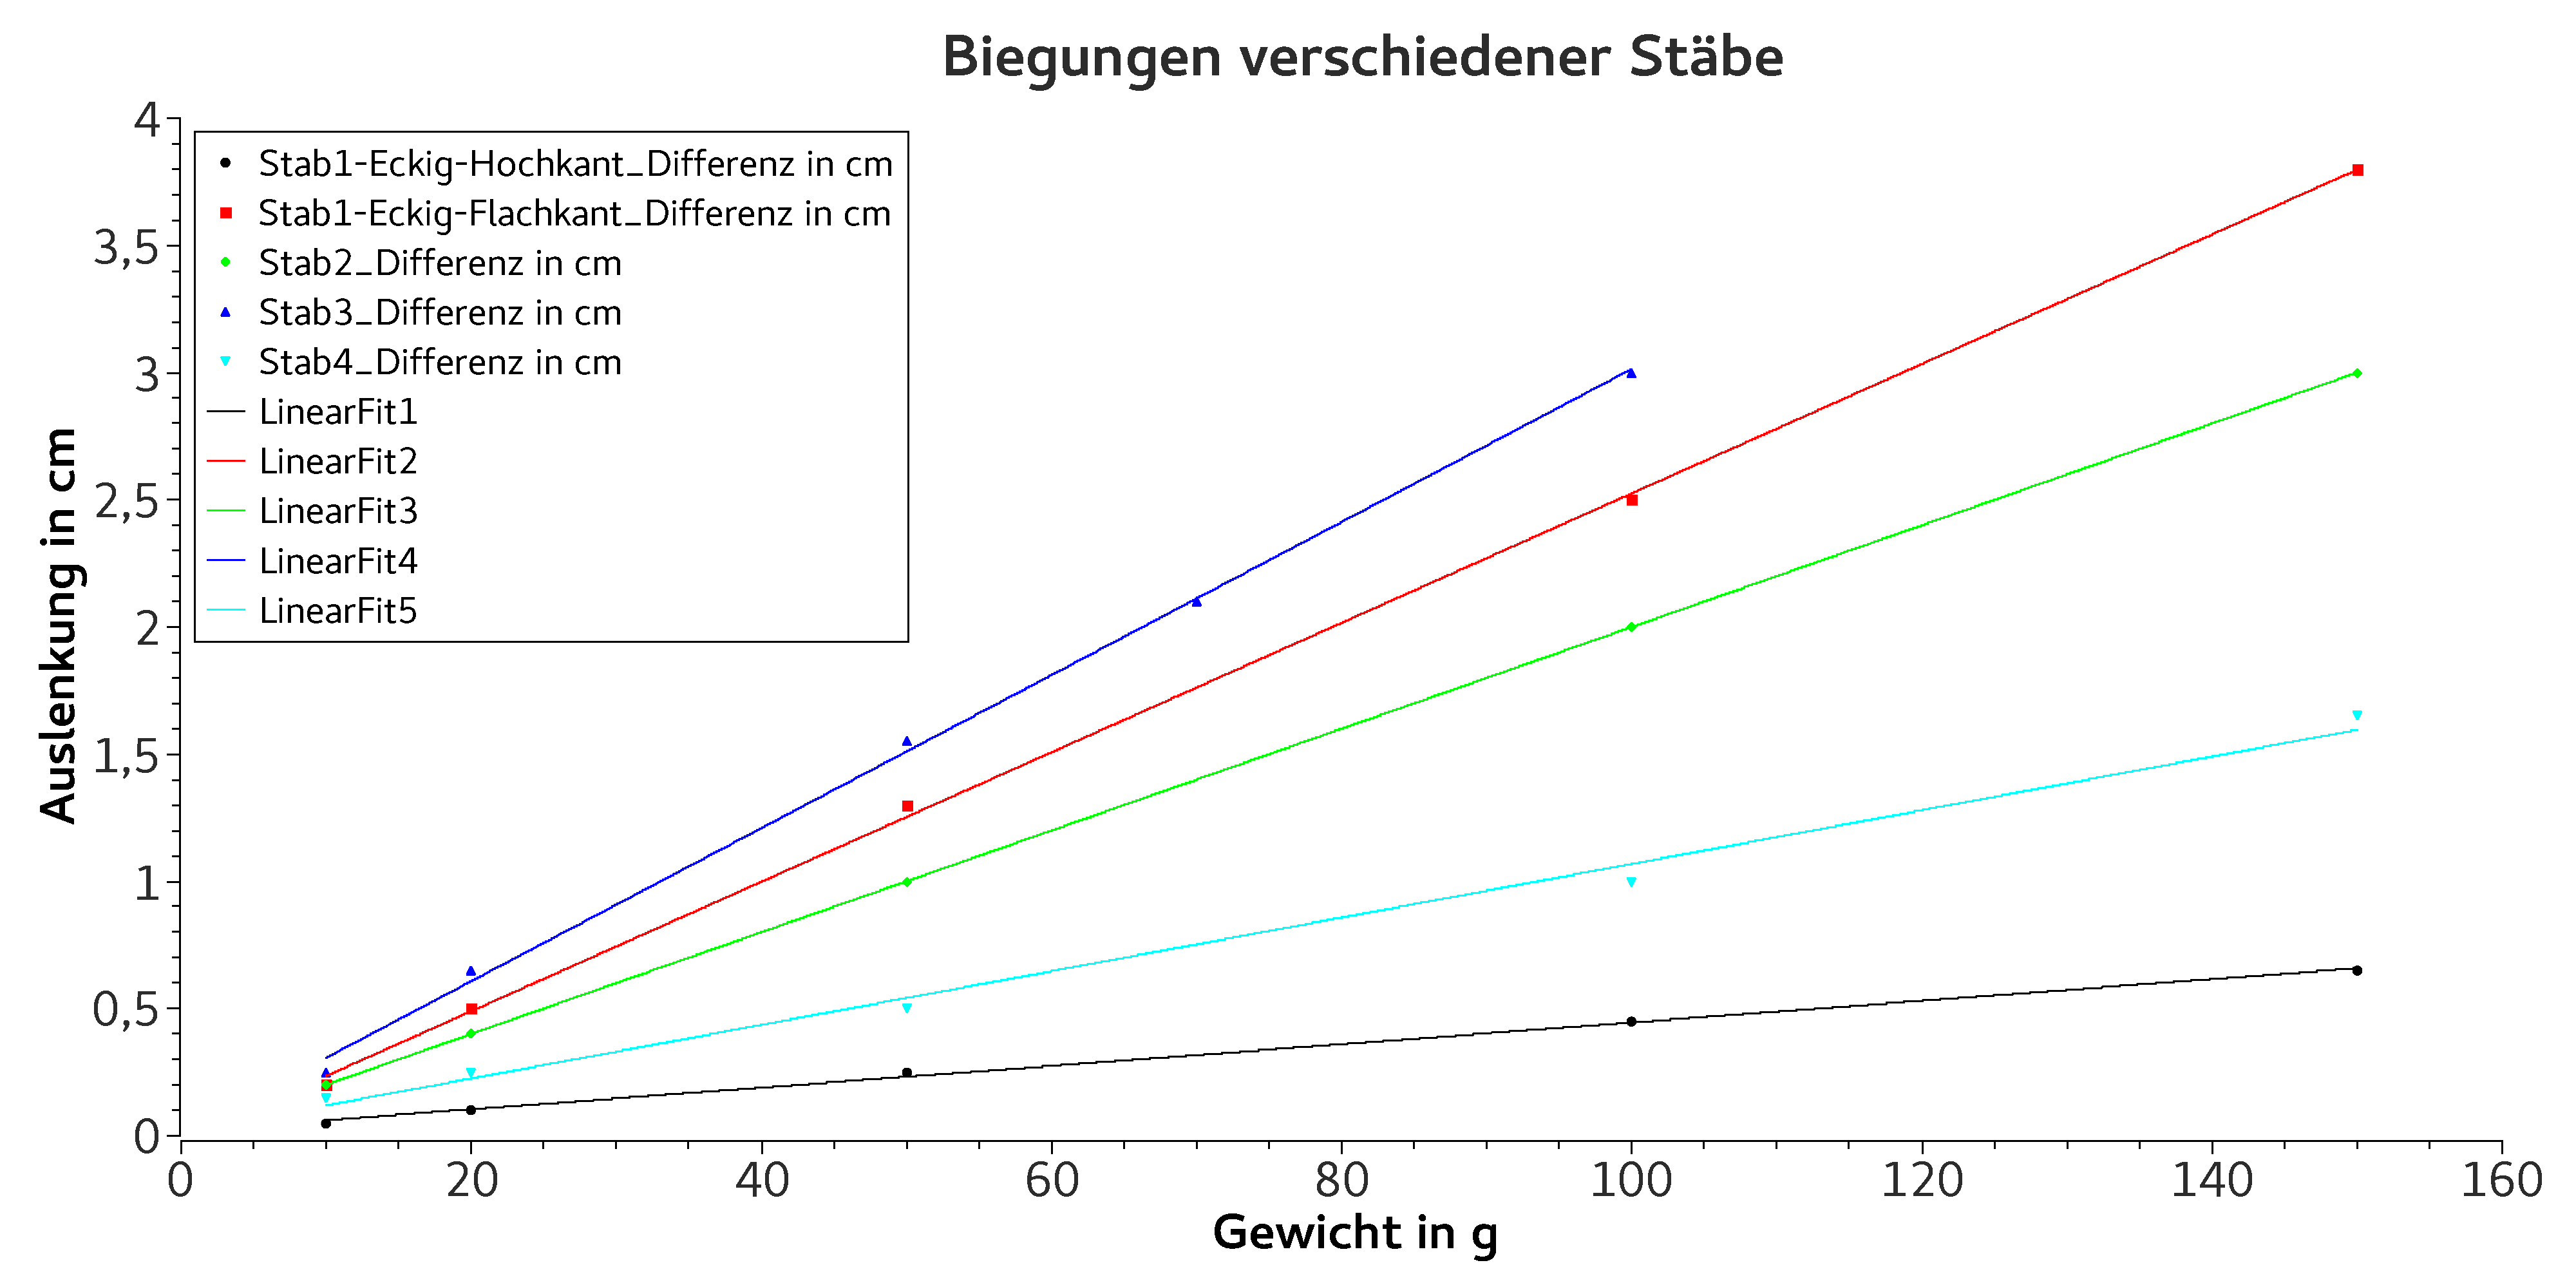
\includegraphics[width=1\textwidth]{Biegungen}
		\centering
		\caption{Biegungen verschiedener Stäbe. Die Fehler sind kleiner als die Symbole}
		\label{BiegungGraph}
		\centering
	\end{figure}

	\begin{table}[tb]
	\centering
	\begin{tabular}{ l | c | c | }
		& a in \SI{}{\centi\meter\per\gram} & b in \SI{}{\centi\meter} \\ \hline %TODO mikro milli und co

		S1 hochkant & $\SI{0,004264 \pm 0,0001}{}$& $\SI{0,018586 \pm 0,01}{}$ \\
		S1 flachkant& $\SI{0,025452 \pm 0,0003}{}$& $\SI{-0,019825 \pm 0,03}{}$ \\ 
		S2 &$ \SI{0,02}{} \pm 6 \cdot 10^{-19}$  &$\SI{0 \pm 5e-17}{}$ \\
		S3 & $\SI{0,030093 \pm 0,0007}{}$ &  $\SI{0,005370 \pm 0,04}{}$\\
		S4 &  $\SI{0,010546 \pm 0,0005}{}$ &$\SI{0,013921 \pm 0,04}{}$  \\ \hline
	\end{tabular}
	\caption{Parameter die sich beim Fitten ergeben}
	\label{TabelleFits}
	\end{table}
	Mit Hilfe von \cref{BiegungGleichung} aus der Einführung des Versuchs lässt sich aus der Steigung der Graphen der Elastizitätsmodul bestimmen. In \cref{TabelleElastizitätsmodule} sind diese aufgelistet.
	Mit Hilfe von \cref{BiegungGleichung} aus der Einführung des Versuchs lässt sich aus der Steigung der Graphen der Elastizitätsmodul bestimmen. In \cref{TabelleElastizitätsmodule} sind diese aufgelistet. Die Unsicherheiten wurden mit \cref{Partielle_Unsicherheiten} berechnet.
	\begin{equation}
		h_{max}= \frac{FL^3}{3EI_\text{q}}
	\end{equation}
	\begin{equation}
		\label{BiegungGleichung}
		E=\frac{gL^3}{3I_\text{q}m}
	\end{equation}
	Wobei $I_\text{q}$ sich wie folgt ergibt:
	\begin{align}
		I_\text{Kreis} = \frac{\pi d^4}{64} \\
		I_\text{Rechteck} = \frac{ab^3}{12}
	\end{align}
	Die Parameter sind $d$ Durchmesser des Stabes, $a$ Rechteckkantenlänge senkrecht zur Biegungsebene und $b$ die verbleibende Rechteckkantenlänge, die nicht Länge des Stabes ist.
	%TODO Fehler/Unsicherheiten
	\begin{table}[tb]
	\centering
	\begin{tabular}{ l | c | c | c |}
		&  $L$ in \SI{}{\meter} & $E$ in $\SI{}{Nm^{-2}}$  \\ \hline
		S1 hochkant & \SI{0,289 \pm 0,00058}{} & \SI{5,383\pm 0,131 e10}{}\\
		S1 flachkant& \SI{0,289 \pm 0,00058}{} & \SI{4,413\pm 0,107e10}{} \\ 
		S2 &\SI{0,285 \pm 0,00058}{} &\SI{1,04\pm 0,03e11}{} \\
		S3 &\SI{0,290 \pm 0,00058}{}& \SI{6,882\pm 0,167e10}{} \\
		S4 &\SI{0,2905 \pm 0,00058}{} & \SI{1,975\pm 0,0485e11}{} \\ \hline
	\end{tabular}
	\caption{Berechnete Elastizitätsmodule}
	\label{TabelleElastizitätsmodule}
	\end{table}
	
	\begin{equation}
	u(y) = \sqrt{  \sum_{i=0}^{N} \left( \frac{\partial f}{\partial x_i}u(x_i)\right)^2  }
	\label{Partielle_Unsicherheiten}
	\end{equation}
	
	\subsubsection{Torsion des Drahtes}
	\subsubsection*{Bestimmung des Schubmoduls}
	Die von uns bestimmte gemittelte Schwingungsdauer der Scheibe beträgt $T=\SI{32,45 \pm 0,04}{s}$.
	Der Schubmodul des Drahtes lässt sich aus gegebener \cref{SchubmodulGleichung} berechnen.
	\begin{equation}
		\label{SchubmodulGleichung}
		G = \frac{4\pi Lm_zR_z^2}{R^4T^2}
	\end{equation}
	Die im Weiteren benötigten Werte wurden ermittelt. 
	\begin{itemize}
		\item $T=\SI{32,45 \pm 0,04}{s}$
		\item $L = \SI{1,8105 \pm 0,0016 }{m}$
		\item $m_z = \SI{2,648}{kg}$
		\item $R_z = \SI{7,325 \pm 0,029}{cm}$
		\item $R = \SI{0,25 \pm 0,0029}{mm}$
	\end{itemize}
	Einsetzten ergibt ein Schubmodul $G$ von $\SI{7,8587\pm 0,3706e10}{Nm^{-2}}$. Dabei folgte die Unsicherheit wieder aus \cref{Partielle_Unsicherheiten}.
	Die Unsicherheiten der Längen ergeben sich aus den Unsicherheiten des Maßbandes bzw. der Mikrometerschraube und die der Schwingungsdauer aus der kombinierten Unsicherheit durch die Digitalanzeige der Stoppuhr und der Reaktionszeit des Menschen. Letztere verringert sich um den Faktor $1/N $ für N gemessene Schwingungsperioden.
	\subsubsection*{Bestimmung des Trägheitsmoments}
	In \cref{TorsionGraph} sind für 5 verschiedene Hanteln die Quadrate der Schwingdauer gegen den Radius der Hanteln aufgetragen. Der lineare Zusammenhang ist beim Betrachten der Werte bereits erkennbar und außerdem sollte dieser der Theorie zufolge auftreten. %TODO Theorie nennen
	Deshalb haben wir einen Fit mit dem \enquote{Scaled Levenberg-Marquardt}-Algorithmus, welcher die Methode der kleinsten Quadrate verwendet, durchgeführt. Die Fit-Funktion sollte wie folgt aussehen:
	\begin{equation}
		f(x)=A*x+B
	\end{equation}
	\begin{figure}[tb]
		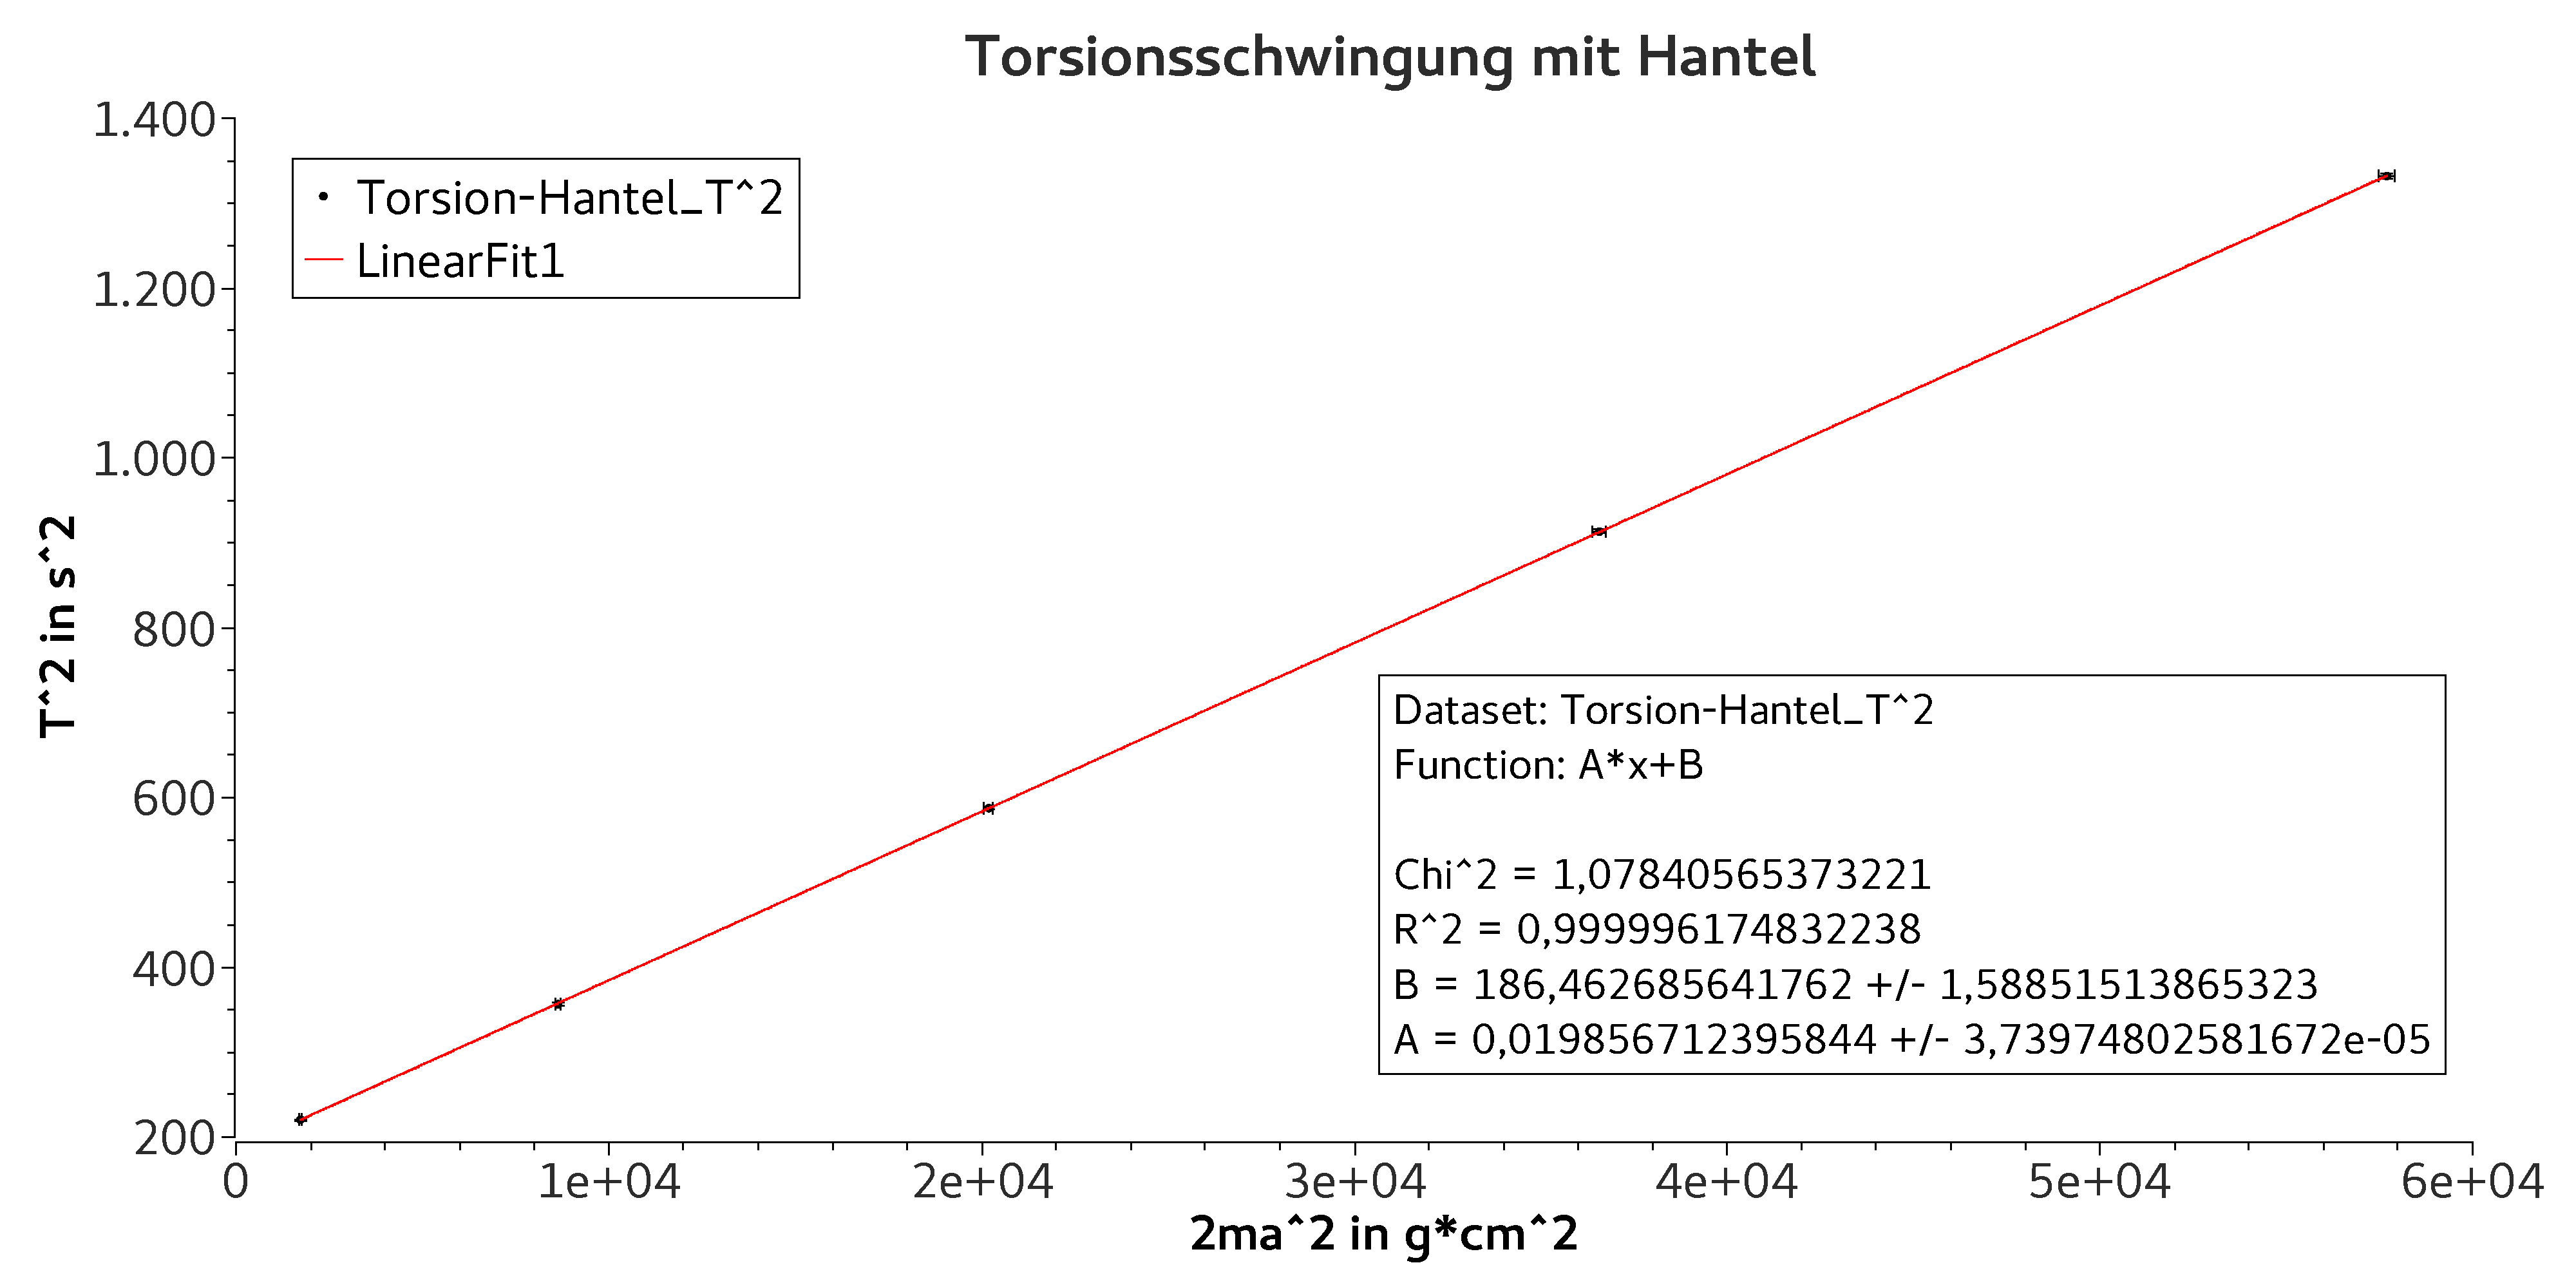
\includegraphics[width=1\textwidth]{Torsion}
		\centering
		\caption{Torsion eines Drahtes mit verschiedene Hanteln. Die Fehler sind kleiner als die Symbole}
		\label{TorsionGraph}
		\centering
	\end{figure}
	Mit Hilfe von \cref{TorsionGleichung} aus der Einführung des Versuchs lässt sich aus der Steigung der Graphen der Direktionsmoment bestimmen.
	\begin{equation}
		\label{TorsionGleichung}
		T^2 = \frac{4\pi^2}{D^*} (J_1 + 2J_2 + 2m_2 a^2)
	\end{equation}
	Das Direktionsmoment ergibt sich mit $m=\SI{0,019857}{s^2g^{-1}cm^{-2}}$ aus:
	\begin{equation}
	D^* = \frac{4\pi^2}{m} = \SI{0,000198814\pm 0,000000374}{Nm} %TODO mikro milli und co
	\end{equation}
	Das Trägheitsmoment der Hantelachse lässt sich aus \cref{TorsionGleichung} mit $J_2=0$, $m_2=0$ und $T=\SI{13,32 \pm0,039}{s}$ berechnen.
	\begin{equation}
		J_1= \frac{T^2D^*}{4\pi^2} = \SI{0,0008935 \pm ,0000055}{kgm^2}
	\end{equation}
	Aus dem Fit in \cref{TorsionGraph} kann man den y-Achsenabschnitt der Gerade ablesen ($T^2$). Dieser entspricht \cref{TorsionGleichung} mit $2m^2a=0$. Setzt man die zuvor berechneten Werte ein, erhält man das Trägheitsmoment der Hantelscheiben $J_2$. %ist meine Ergänzung true?
	\begin{equation}
		J_2 = \frac{T^2D^*}{8\pi^2} - \frac{J_1}{2} = \SI{0,00002276 \pm 0,00000493}{kgm^2}
	\end{equation}

	Die Trägheitsmomente der Hantelscheibe und der Hantelachse lassen sich auch direkt aus ihrem Gewicht und ihrer Form berechnen.
	\begin{align}
		J_1 = m_1(\frac{1}{12}l_1^2+\frac{1}{4}r_1^2) = \SI{0,00115 \pm0,00001}{kgm^2}\\
		%\label{Form_Hantelachse_Trägheits_Moment}
		J_2 = m_2(\frac{1}{12}l_2^2+\frac{1}{4}(r_2^2 + r_1^2))= \SI{0,0000594\pm 0,0000091}{kgm^2}
		%\label{Form_Hantelscheibe_Trägheits_Moment}
	\end{align}
	
	\subsection{Diskussion}
	Zunächst stellen wir folgende Vermutungen für die Materialien der Stäbe auf: Stab 1 und Stab 2 bestehen nach Farbe und Gewicht zu urteilen vermutlich aus Messing (goldfarben, aber weniger schwer als Gold). Stab 3 ist recht leicht und silbrig gefärbt. Daraus schließen wir, dass er wohl aus Aluminium besteht. Stab 4 ist schwerer und dunkler gefärbt, was die Vermutung aufkommen lässt, dass es sich um einen Stahl handelt. Daraus ergeben sich die in \cref{Tabelle_Elastizitätsmodule_Literatur} dargestellten Erwartungen für die Elastizitätsmodule der Stäbe. Ebenfalls aus Stahl besteht vermutlich der Torsionsdraht, der eine ähnliche Färbung wie Stab 4 aufweist. Da wir nicht wissen, um welche Art von Stahl es sich handelt, können wir auch nur eine ungenaue Erwartung für den Schub- und Elastizitätsmodul aufstellen. Wir verwenden hierfür den Elastizitätsmodul von Baustahl.
	
	\begin{table}[tb]
		\centering
		\begin{tabular}{ r | c | c | c |}
			&  Messing & Aluminium& Stahl\\ \hline
			Elastizitätsmodul /\si{\giga \pascal} & 78…123 & 70 & 210\\
			Schubmodul /\si{\giga \pascal} & & & 79,3 \\
			\hline
		\end{tabular}
		\caption{Literaturwerte der Elastizitätsmodule der Materialien, aus denen die Stäbe und der Torsionsdraht vermutlich bestehen und das Schubmodul von Stahl. Aluminium und Baustahl aus ~\cite[S. 624 f.]{Taschenbuch} und Messing aus ~\cite[S. E 66.]{Huette} sowie der Schubmodul von Stahl~\cite{Solids}} %vlt bissl schöner verpacken
		\label{Tabelle_Elastizitätsmodule_Literatur} 
	\end{table}
	
	Wenn man die Literaturwerte (\cref{Tabelle_Elastizitätsmodule_Literatur}) der Elastizitätsmodule mit den gemessenen (\cref{TabelleElastizitätsmodule}) vergleicht, stellt man fest, dass zwar Abweichungen existieren, die zum Teil auch größer als die Unsicherheiten sind, aber insgesamt sich doch unsere Vermutungen bestätigen lassen. Speziell fällt auf, dass die flachkantige Messung von Stab 1 einen anderen Wert für das Elastizitätsmodul ergibt als die hochkantige, was eigentlich nicht zu erwarten ist. Diese Abweichungen lassen sich darauf zurückführen, dass die Stäbe keine exakten Zylinder bzw. Quader waren, sondern schon eine gewisse Verformung der Stäbe vorhanden war. Außerdem wurden die angehängten Gewichte als exakt angenommen. Wie präzise diese Annahme ist, ist nicht bekannt. Auch ist nicht zu vergessen, dass Messing eine Legierung ist und somit genauso wie Stahl unterschiedlich zusammengesetzt sein kann. %TODO Tabelle? kein bock
	\\
	\par
	Die Literatur gibt für den Schubmodul von Stahl \SI{79,3}{\giga \pascal}(\cref{TabelleElastizitätsmodule}) an. Dies unterscheidet sich von dem gemessenen Wert von \SI{78,587\pm 0,03706e10}{\giga \pascal} nur geringfügig, aber um mehr als die Unsicherheit unserer Messung. Diese lichte Abweichung kann mit der nicht exakt mittigen Aufhängung der Scheibe und dem nicht exakt zylinderförmigen Draht zusammenhängen, lässt aber darauf schließen, dass der Draht vermutlich tatsächlich aus Stahl bestand.
	\par
	\begin{table}[tb]
		\centering
		\begin{tabular}{ r | c | c |}
			Trägheitsmomente (\si{kgm^2})& aus Torsionsgleichung & aus Form und Masse\\ \hline
			Hantelachse & $0,0008935 \pm ,0000055$ &$ 0,00115 \pm0,00001$\\
			Hantelscheiben & $0,00002276 \pm 0,00000493$ & $0,0000594\pm 0,0000091$\\ \hline
		\end{tabular}
		\caption{Die Trägheitsmomente, die aus der Torsionsgleichung berechnet wurden, verglichen mit denen, die aus Form und Masse berechnet wurden}
		\label{Trägheitsmomente_Vergleich} 
	\end{table}
	
	Wenn man wie in \cref{Trägheitsmomente_Vergleich} die Trägheitsmomente aus der Torsionsgleichung mit denen aus Form und Masse vergleicht, stellt man fest, dass die Abweichungen deutlich größer als die Unsicherheiten sind. Dies lässt sich möglicherweise darauf zurückführen, dass die Hantel nicht exakt in der Mitte aufgehängt werden konnte, da der Torsionsdraht nicht exakt in der Mitte der Schraube, mit der er mit der Hantel verbunden war, befestigt war. Außerdem wurde der Draht als perfekter Zylinder angenommen, während er in der Realität einige Knicke aufwies. Zuletzt ist noch zu bemerken, dass Stahl unterschiedliche Zusammensetzungen und somit unterschiedliche  Elastizitätsmodule haben kann.
	
	\section{Schlussfolgerung}
	Die durchgeführten Messungen haben eine Bestimmung der Elastizitäts- bzw. Schubmodule erlaubt.
	Bei der Untersuchung des Elastizitätsmoduls verschiedener Stäbe konnten die ersten Vermutungen bezüglich des Materials der Stäbe innerhalb annehmbarer Wahrscheinlichkeiten bestätigt werden.
	Dann konnte das Schubmodul des Torsionsdrahtes bestimmt werden, was ein Ergebnis lieferte, dass die Vermutung, es handle sich bei dem Draht um Stahl, bestätigte.
	Alle Messungen, die mit einem Maßband durchgeführt wurden, waren insofern erschwert, als dass bei allen zur Verfügung stehenden Maßbändern das metallene Endstück nicht mehr korrekt genietet war, weshalb dieses Endstück per Hand zusammengehalten werden musste.
	\printbibliography
\end{document}
